%!TEX root = ../../csuthesis_main.tex
\title{基于数字孪生的自动驾驶强化学习仿真系统}

\chapter{绪论}



\section{研究背景及意义}

\subsection{自动驾驶技术的发展历程}

汽车作为传统交通工具的一员,汽车为人们的出行带来了极大的便利,随着中国国民经济不断高速发展,国内汽车的生产销售量节节高升。根据中央数据显示,2023年全国机动车保有量达4.35亿辆,其中汽车3.36亿辆。目前机动车驾驶人达5.23亿人,其中汽车驾驶人4.86亿人。汽车保有量的增加给交通带来了一系列挑战,诸如道路拥堵、交通安全以及城市规划等方方面面的挑战。首先,道路拥堵成为了常见现象,这不仅浪费了人们宝贵的时间,还增加了通勤的压力,同时也大大增加了交通事故的风险。另外,交通事故也是一个严重的问题,这导致了人员伤亡和财产损失,专
门的研究显示,超过百分之九十的交通事故都是由于驾驶员的不当驾驶操作导致的,其中包括了超速、酒驾、疲劳驾驶、分心驾驶(如使用手机)、违反交通规则等,这些行为不仅降低了驾驶员对道路的控制能力\cite{关鑫2023自动驾驶安全挑战},而且增加了事故发生的风险。

然而随着科技的蓬勃发展,自动驾驶(AD)技术的出现为解决这些问题带来了新的希望和机遇。自动驾驶,又称无人驾驶,是指车辆无需人类引导,能够感知和行驶周围环境,确定最佳行驶路线,顺利到达目的地。自动驾驶技术根据自主程度分为六个级别,从纯人工控制的L0到完全自主控制的L5,如表1-1所示。 L4、L5级别表示车辆可以在无需特定条件、无需人工干预的情况下完全自主行驶,代表着最高的技术水平\cite{1023549446.nh}。


\begin{table}[htbp]
	\centering
	\caption{自动驾驶等级对照表}
	\label{tab:driving-levels}
	\begin{tabular}{ccccccc}
		\toprule
		\textbf{等级} & \textbf{名称} & \textbf{驾驶操作} & \textbf{周边监控} & \textbf{接管} & \textbf{应用场景} \\
		\midrule
		L0   & 人工驾驶      & 人类驾驶员 & 人类驾驶员 & 人类驾驶员 & 无 \\
		L1   & 辅助驾驶      & 车辆与人类 & 人类驾驶员 & 人类驾驶员 & 有限场景 \\
		L2   & 部分自动驾驶  & 车辆       & 人类驾驶员 & 人类驾驶员 & 有限场景 \\
		L3   & 条件自动驾驶  & 车辆       & 车辆      & 人类驾驶员  & 有限场景 \\
		L4   & 高度自动驾驶  & 车辆       & 车辆      & 车辆       & 有限场景 \\
		L5   & 全自动驾驶    & 车辆       & 车辆      & 车辆       & 所有场景 \\
		\bottomrule
	\end{tabular}
\end{table}

我们可以发现自动驾驶技术的发展历程可以追溯到20世纪中叶,伴随着计算机科学、传感器技术以及控制理论
的不断进步,自动驾驶逐渐从理论研究走向实际应用。早期的自动驾驶研究主要集中在简单的路径
跟踪和基本的环境感知上,这些技术虽然在当时具有一定的前瞻性,但由于计算能力和传感器精度
的限制,实际应用效果并不理想。赵岑等人指出,随着人工智能和大数据技术的引入,自动驾驶的智
能化水平显著提升,使得车辆能够在复杂环境中进行自主决策,从而推动了整个行业的快速发展\cite{小龙刘2024人工智能和大数据技术在自动驾驶中的应用}。
进入21世纪,深度学习的快速发展为自动驾驶技术带来了新的机遇。基于深度学习的端到端自
动驾驶系统能够实现更高效的决策与控制,极大地推动了行业的进步。这种方法通过大规模的数据
训练,使得自动驾驶系统能够在多种驾驶场景中进行有效的学习和适应,显著提高了自动驾驶的安
全性和可靠性。随着科技的迅猛发展,自动驾驶技术逐渐成为交通运输领域的研究热点\cite{丘德龙2018浅谈人工智能在汽车领域中的应用}。近年来,
数字孪生技术的兴起为自动驾驶系统的开发与优化提供了新的思路和方法。数字孪生是指通过虚拟
模型实时反映物理实体的状态和行为,能够在仿真环境中进行多种场景的测试与验证\cite{罗健炜2023基于数字孪生的自动驾驶仿真测试研究}。这一技术的
应用,不仅可以降低实际测试中的风险和成本,还能加速自动驾驶算法的迭代与优化。

在自动驾驶的研发过程中,强化学习作为一种重要的机器学习方法,能够通过与环境的交互不
断提升系统的决策能力。传统的强化学习往往依赖于大量的真实数据和复杂的环境模拟,这在实际
操作中面临诸多挑战。基于数字孪生的自动驾驶强化学习仿真系统,能够提供一个高度真实且可控
的虚拟环境\cite{梁恩云2021基于数字孪生的自动驾驶交通场景构建研究},使得研究人员可以在不同的交通场景和复杂情况下进行训练,从而提高算法的鲁棒性
和适应性。

近年来,自动驾驶技术的应用逐渐扩展到商用领域,通过分析智能自动驾驶无人机的技术进展,
为这一领域的创新为传统交通运输方式带来了颠覆性的变革\cite{方韶剑2024基于深度学习的智能自动驾驶无人机技术分析}。汽车的自动驾驶技术不仅提升了物
流效率,还在应急救援、环境监测等领域展现了广泛的应用潜力。强化学习作为一种重要的机器学
习方法,逐渐被应用于自动驾驶决策中。研究者研究了基于强化学习的无信号交叉口自动驾驶决策\cite{李文娜2024自动驾驶汽车闯红灯预警数字孪生道路测试},
指出该方法能够有效提高车辆在复杂交通场景中的决策能力,尤其是在动态变化的环境中。通过探
讨多源数据在自动驾驶技术风险识别中的应用,突出强调了数据驱动方法在提升自动驾驶安全性方
面的重要性。总的来看,自动驾驶技术的发展历程是一个不断融合多学科知识、不断创新的过程,
未来将继续朝着更高的智能化和安全性方向迈进,推动交通运输领域的革命性变革。







\subsection{数字孪生技术的概念与应用}

“孪生”的概念起源于美国国家航空航天局的“阿波罗计划”,即构建两个相同的航天飞行器,
其中一个发射到太空执行任务,另一个留在地球上用于反映太空中航天器在任务期间的工作状态,
从而辅助工程师分析处理太空中出现的紧急事件。当然,这里的两个航天器都是真实存在的物理实
体。“数字孪生”初始的概念模型是于2002年10月由迈克尔·格里弗斯(Michael Grieves)博士
在美国制造工程协会管理论坛上所提出。而到2009年,美国空军相关实验室明确提出带有数字孪生
的概念:“机身数字孪生(Airframe Digital Twin)”。在2010年,美国国家航空航天局(NASA)
在《建模、仿真、信息技术和处理》和《材料、结构、机械系统和制造》两份技术路线图中正式开
始使用数字孪生(Digital Twin)这一名称。


数字孪生技术也称作数字双生、虚拟双生或者数据双生,它是一项可在虚拟空间里模拟、优化并复制物理实体的技术,借助数字孪生技术,现实中的物体、系统或过程可在虚拟环境中得以模拟呈现,基于此,人们运用数字孪生技术对虚拟环境中的物体实施实时监测、优化以及预测,近年来,人们察觉到数字孪生技术在自动驾驶领域有优势\cite{王庆涛2021数字孪生技术在自动驾驶测试领域的应用研究概述}。借助该技术,人们可构建虚拟环境用以训练和测试自动驾驶系统,这有效降低了自动驾驶模型训练的时间与成本,同时保障了训练和测试自动驾驶模型时的安全\cite{葛雨明2020基于数字孪生的网联自动驾驶测试方法研究},而且人们可在虚拟环境中设定一些现实生活里较难达成的场景,以此训练自动驾驶模型在各类复杂情形下的稳定性与可靠性。为自动驾驶系统在复杂状况下的运行提供了参考样本。

数字孪生技术用于自动驾驶领域,可优化自动驾驶车辆性能,提升自动驾驶系统对周围环境的敏感度,提高自动驾驶车辆的环境感知能力,这能让自动驾驶车辆精准了解周边环境,提高其安全性\cite{覃熊艳2024关于},随着新一代信息技术快速发展,数字孪生技术在车辆上实施渐成可能,如今能看到数字孪生技术已在诸多领域广泛应用,像电力、船舶、城市管理、农业、建筑、制造、石油天然气、健康医疗、环境保护等行业。在这些行业取得了不错成果,在智能制造领域,数字孪生技术被视作实现虚拟世界与现实世界交互的有效办法,不少知名企业和组织都高度重视数字孪生技术,且积极探索其在各领域的应用,把数字孪生技术与强化学习结合,可利用数字孪生技术提供的虚拟环境训练和测试自动驾驶系统模型,降低模型训练风险,又大幅提升自动驾驶模型应对复杂情况的稳定性和可靠性\cite{马帅2024基于深度学习的汽车自动驾驶控制系统测试方法研究}。数字孪生技术与强化学习结合的思路为自动驾驶系统发展提供了新方向,依靠数字孪生技术实时提供的数据随时调整和更新模型,使自动驾驶模型面对复杂现实交通场景时能更灵活应对\cite{赵恩波 于家旺 王晓鹏 曲强2023深度学习在自动驾驶汽车中的应用},数字孪生技术应用于自动驾驶领域,可提升自动驾驶系统智能化水平,提高自动驾驶系统决策准确性。


\subsection{强化学习在自动驾驶中的重要性用}

强化学习作为深度学习的一种方法,在诸多应用领域都有广泛运用,该方法使代理可尝试各种不同行为,观察行为所产生的结果,并依据奖励信号来调整自身策略,以此达成最大化预期奖励这一目标,强化学习有适应复杂且不确定环境的能力,可自动作出决策,同时对持续的活动以及公共空间给予监控,且无需依赖手动数据。基于此,强化学习算法在自动驾驶、机器人、医疗器械、无人机等众多领域均有广泛应用。

在自动驾驶不断发展的进程中,强化学习算法起到了极为关键且不可替代的作用,强化学习算法作为机器学习算法里颇为关键的一种,在各个不同领域都有广泛应用,在自动驾驶领域内,强化学习算法借助持续与周边环境展开交互,以此对模型给予调整,让自动驾驶系统的模型更契合人们对它的需求。正是强化学习算法这种依靠与周围环境交互来学习的特性,为自动驾驶系统赋予了相较于其他机器学习算法更强的灵活性与适应性,自动驾驶模型借助强化学习算法获得了可更灵活应对各类复杂交通状况的能力\cite{韩胜明2023深度强化学习在自动驾驶系统中的应用综述},采用端到端的深度强化学习方法,能发现它有效提升了自动驾驶模型的灵活性,还大幅降低了自动驾驶模型的复杂性。这让我们可更快训练出符合需求的模型,也促使自动驾驶技术得以广泛应用于各种复杂交通场景\cite{魏兆吉2021端到端免模型深度强化学习在自动驾驶中的应用研究}。

凭借强化学习算法可训练自动驾驶模型,自动驾驶模型能于虚拟仿真环境中获取大量源于现实数据的仿真训练,这让强化学习算法在虚拟仿真环境里得到充分训练\cite{梁恩云2022面向自动驾驶仿真测试的数字孪生场景交互研究与实现},积累丰富经验优化自动驾驶系统决策,自动驾驶系统决策优化后,面对复杂场景能以更短时间做出出色决策避免危险,使其能更从容应对未知环境。现有各项研究显示强化学习算法在自动驾驶中的关键性,体现在提升决策能力方面,还为系统持续优化及适应复杂环境提供有力支持。


\section{文献综述}

\subsection{国内研究现状}

近些年来,随着自动驾驶技术快速发展,国内学者针对数字孪生技术在自动驾驶领域的应用展开了广泛且深入的研究,数字孪生技术的汽车自动驾驶仿真测试方法可有效提升测试安全性与效率,为自动驾驶系统验证带来新的思路及方法,此方法能模拟真实驾驶环境,又能于虚拟空间开展多种场景测试,以此降低实际测试中的风险与成本\cite{文谢2023基于数字孪生的汽车自动驾驶仿真测试方法}。经探讨数字孪生技术的虚拟仿真系统,能发觉其在复杂驾驶环境下的应用潜力,研究说明数字孪生技术可为自动驾驶提供更真实测试环境,提升自动驾驶系统的可靠性与适应性\cite{彭博2023基于数字孪生的虚拟仿真系统研究与应用},学者李佳新等人在研究中深入探讨深度强化学习在自动驾驶领域的应用,并提出一种新型决策框架,该决策框架可有效提高自动驾驶系统的智能化水平。关注端到端免模型深度强化学习的应用,能发现此方法在复杂交通环境中的优势,可自动驾驶系统实现更灵活驾驶,深入研究深度学习与深度强化学习结合技术,能发现这种结合可提升自动驾驶系统的感知与决策能力,学者何竞等人提出一种基于深度强化学习的智能决策算法,强调该算法在动态环境下的适应性与实时性。探讨自主无人系统的驾驶策略,学者们提出一种新的强化学习框架,该学习框架能有效应对复杂驾驶场景,学者李文娜\cite{李文娜2024自动驾驶汽车闯红灯预警数字孪生道路测试}等人研究自动驾驶汽车闯红灯预警的数字孪生道路测试,强调数字孪生技术在提升自动驾驶安全性方面的关键作用,仿真测试对自动驾驶系统开发非常关键,可有效降低开发成本与风险。

国内研究者凭借综述自动驾驶汽车感知系统的仿真研究,指出数字孪生技术在感知系统优化中的关键作用,学者们研究自动驾驶汽车闯红灯情况下的预警机制,提出数字孪生技术进行道路测试可提高系统的反应能力与决策准确性,这一研究为自动驾驶系统的安全性提供关键理论支持与实践依据。国内学者分析仿真测试在自动驾驶系统开发中的关键性,发现仿真可有效降低开发成本与时间,提高系统的可靠性与稳定性,加速自动驾驶技术的落地与应用\cite{杨海清2024仿真测试在自动驾驶系统开发中的重要性}。

国内有研究者开展了基于转鼓/制动试验平台的自动驾驶整车虚拟仿真测试系统\cite{田常青2024基于转鼓}的设计工作,着重体现了数字孪生技术于整车测试中的应用价值,证实了该技术在实际工程里有可行性与有效性,从中可看出数字孪生技术在汽车行业的应用进程不断加速,于智能工厂以及自动驾驶领域,呈现出广阔的前景与发展潜力\cite{高驰2023智能工厂}。随着数字孪生技术在自动驾驶测试领域应用研究的推进,其可为未来技术发展筑牢根基,国内研究者在数字孪生与自动驾驶结合的研究方面已获一定成果,不过仍需持续探索与实践,以应对变得日益复杂的驾驶环境和技术挑战。

\subsection{国外研究现状}
我们可观察到,在国外,自动驾驶技术的研究跟应用已然取得了一定进展,在数字孪生技术与强化学习相结合这方面,不少知名的科技公司以及研究机构都在踊跃投入资源,探寻怎样借助数字孪生技术来提高自动驾驶系统的性能以及安全性,像特斯拉、谷歌的Waymo以及Uber等公司,都在其自动驾驶平台里运用了先进的仿真技术,以此来应对复杂的交通环境以及多样化的驾驶场景。另外许多国际知名高校和研究机构,例如麻省理工学院、斯坦福大学以及卡内基梅隆大学等,都在这个领域开展了相关研究,数字孪生技术的引入,让研究者可在虚拟环境中创建和现实世界极为相似的环境模型,为自动驾驶系统的开发与测试给予了有力支持,

我们可发现,在数字孪生技术的研究过程中,国外学者提出了多种构建及应用模型。MIT的研究团队研发出了一种基于数字孪生的城市交通仿真平台,该仿真平台可以实时呈现城市交通流量以及车辆行为,这个平台为自动驾驶算法的测试提供了真实的环境数据,还为城市交通的管理提供了决策方面的支持,斯坦福大学的研究者们也在探索数字孪生在自动驾驶中的应用,他们着重关注如何凭借高保真度的仿真环境来优化车辆的决策过程。

人们都清楚,世界上第一辆无人驾驶汽车“Linrrican Wonder”于1925年在美国纽约诞生,在2004年至2007年这段时间里,美国接连举办了三届DARPA无人驾驶挑战赛,此举意味着自动驾驶时代正式开启,无人驾驶挑战赛的以便促进极端环境下自动驾驶汽车技术向前发展,参赛队伍包含了许多高校以及高科技企业。无人驾驶挑战赛主要运用的技术涉及了人工智能、计算机技术、汽车设计等众多高科技领域,每一届比赛都对自动驾驶汽车技术的发展起到了较大的推动作用,2004年,首届DARPA挑战赛在美国哈维沙漠举办,尽管参赛队伍都没能完成比赛规定的任务,不过这是车辆首次可在自动驾驶时实现避障,这极大地激发了人们对自动驾驶技术的热情,提高了自动驾驶领域的创新意识,对自动驾驶的发展有着里程碑式的意义。和第一届DARPA无人驾驶挑战赛相比,2005年的第二届DARPA比赛中,虽然车辆配备了大量传感器,但部分队伍已采用线控技术来控制车辆,这是一个重大的进步,第二届挑战赛形成了自动驾驶汽车的初步形态,标志着自动驾驶汽车的功能基本完善,五辆赛车完成了全部比赛任务,证明了自动驾驶是可行的。2007年,DARPA城市挑战赛在加州一个废弃的空军基地举行,跟前两届比赛相比,本届比赛最大的亮点在于自动驾驶汽车要避让其他机动车辆,还要遵守道路交通规则,这对车辆的感知系统和决策能力是一个巨大的挑战。

在智能汽车领域,能观察到谷歌于2009年着手无人驾驶汽车项目研究,2012年,Google Auto获得由美国内华达州颁发的美国历史上首张自动驾驶牌照,2014年,谷歌宣称其自动驾驶汽车可应对数千个城市的道路交通,还发布了第三代自动驾驶汽车,此款车是谷歌自主研发的纯电动自动驾驶汽车,没有传统汽车的刹车、方向盘与油门。2016年5月,谷歌与克莱斯勒汽车公司开启首次合作,该车配备了全套传感器、信息处理计算单元等系统,2016年12月,谷歌成立无人驾驶公司Waymo,并对外展示一款自动驾驶概念车,该车顶部装有激光雷达和摄像头装置,前后保险杠处安装了传感器,截至2016年3月,谷歌的自动驾驶里程已达241万公里,这期间仅发生14起交通事故,其中13起\cite{janai2020computer}是由对方失误导致。截至2017年底,谷歌的自动驾驶汽车测试里程已达141.6公里,依据谷歌提供的测试报告,谷歌Waymo每千英里仅需人工干预0.18次,相当于每9000公里约需1次人工干预,排名第二的通用汽车Cruise则需人工干预0.84次,而宝马、奔驰、奥迪、特斯拉等其他国际知名汽车公司,都在开展自动驾驶汽车的研究与测试,各公司之间也在进行相应合作与战略部署。美国于2016年9月发布了《联邦自动驾驶汽车政策》,这是全球首个自动驾驶领域的政策文件\cite{陈燕申2017美国政府},以此推动智能汽车健康规范发展。

可观察到,强化学习技术于自动驾驶领域的应用也受到不少关注,国外研究者借助设计复杂奖励机制与状态空间机制,促使强化学习算法在自动驾驶决策领域得以应用,加州大学伯克利分校研究小组提出一种基于深度强化学习的自动驾驶模型,该模型经与数字孪生环境交互,车辆在复杂场景下的自主决策能力有所提升。此自动驾驶模型在多种仿真测试中的出色表现,呈现出强化学习算法于动态环境中的适应性与灵活性,还可以看到,国外研究者凭借构建复杂仿真环境,运用深度强化学习算法优化自动驾驶决策,DeepMind和OpenAI等机构在强化学习算法创新方面有成果,其研究推动了人工智能发展,为自动驾驶技术进步提供新思路。诸多企业如特斯拉、谷歌的Waymo以及Uber等,纷纷投入大量资金开展自动驾驶技术研发,利用数字孪生技术进行实时数据分析与模型优化,以此提升自动驾驶系统的安全性和可靠性。

可看到,国外研究突出了多智能体系统于自动驾驶里的意义,借助数字孪生技术,研究者可模拟多个自动驾驶车辆于同一环境中的交互行动,给强化学习算法提供更丰富训练数据,国外研究还关注多智能体系统的协同学习,凭借模拟多个自动驾驶车辆于复杂交通环境中的互动,剖析如何提升整体交通效率与安全性。这些研究能为自动驾驶技术的实际应用给予理论支撑,又为未来智能交通系统筑牢了坚实根基,国外在基于数字孪生的自动驾驶强化学习仿真系统研究方面,取得了一定进展,值得学习,国外研究者在数字孪生与强化学习结合的自动驾驶研究中,形成了一定理论基础与实践经验,为推动自动驾驶技术发展奠定了坚实基础。

\section{本文结构框架}
本文首先对研究背景及意义进行了概述,根据目前国内外研究现状综合分析z自动驾驶领域的研究进展,聚焦于基于深度学习的方法与应用,对相关理论进行整理分析。在此基础上,需要特别关注强化学习算法在自动驾驶方面的应用、以及数字孪生技术在自动驾驶领域的应用与研究。

对于特定的自动驾驶流程,本文借助对强化学习算法奖励函数加以调整,促使训练得到的强化学习算法模型契合我们对自动驾驶模型的要求,强化学习算法是依据奖励函数设定实现实时学习的算法,它借助与Carla仿真环境持续交互来训练模型,让模型达到我们的需求,我们可运用构建的自动驾驶系统明晰所训练的自动驾驶模型效果是否符合我们的需求。


\begin{figure}[hbt]
	\centering
	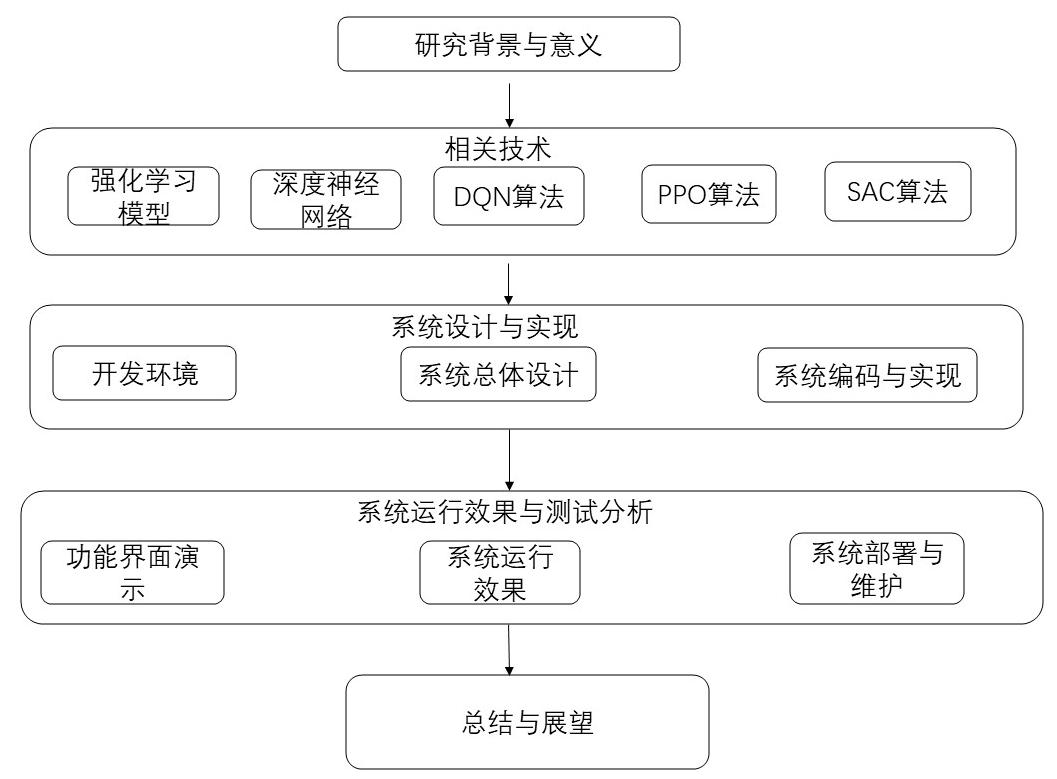
\includegraphics[width=\linewidth]{论文结构框架图.jpeg}
	\caption{论文结构框架图}
	\label{f.example}
\end{figure}



\begin{tabular}{l l}
%  \verb|\songti| & {\songti 宋体} \\
%  \verb|\heiti| & {\heiti 黑体} \\
%   \verb|\kaiti| & {\kaiti 楷体}
\end{tabular}


